\documentclass[thesis.tex]{subfiles}

\begin{document}

\chapter{Evaluation}\label{chap:eva}

This chapter contains the results of the experiments from the different strategies and methods as discussed in \autoref{chap:main}. The experiment shall show if the postulated SpeedCam approach achieves the goals (\autoref{sec:intro:goals}). At first, it describes the test environment so that the experiment is repeatable and the results are verifiable. Then it list the different experiment configuration and lastly their results, which will be interpreted and discussed.

\section{Test environment}
The test environment was the SCIONLab network after its major update on 03.04.2018 and was monitored for 48h. The network is changing over time because user can create a SCIONLab VM and automatically attach them to an existing end point such as 1-17. This enables the user to try out SCION in a virtual environment. A snapshot of the network can be seen in \autoref{fig:eva:scionLabTopo}, which is the topology after a few exploration episodes. It does not represent the complete topology, only the current observed one. 

The inspector program is running on the same machine as the SCPB, while the scripts for information about border router interfaces and path server requests are running on different machines. The inspectors ran on a virtual machine on a Intel i7@3.75 GHz with one assigned core, 1GB of RAM and using a 52GB SSD. On this VM ran also the Prometheus server in version 2.2.1 and a Grafana\footnote{{\url{https://grafana.com/}, 18.04.2018}} in version 5.0.1 for visualizing the. One problem with that test environment was that there weren't border router information for all nodes in the network. This results in fewer usable nodes than there were ASes as seen in \autoref{fig:eva:scionLabTopo}, which results in a lower precision. This has to be considered in the interpretation of the results.

\begin{figure}
	\centering
	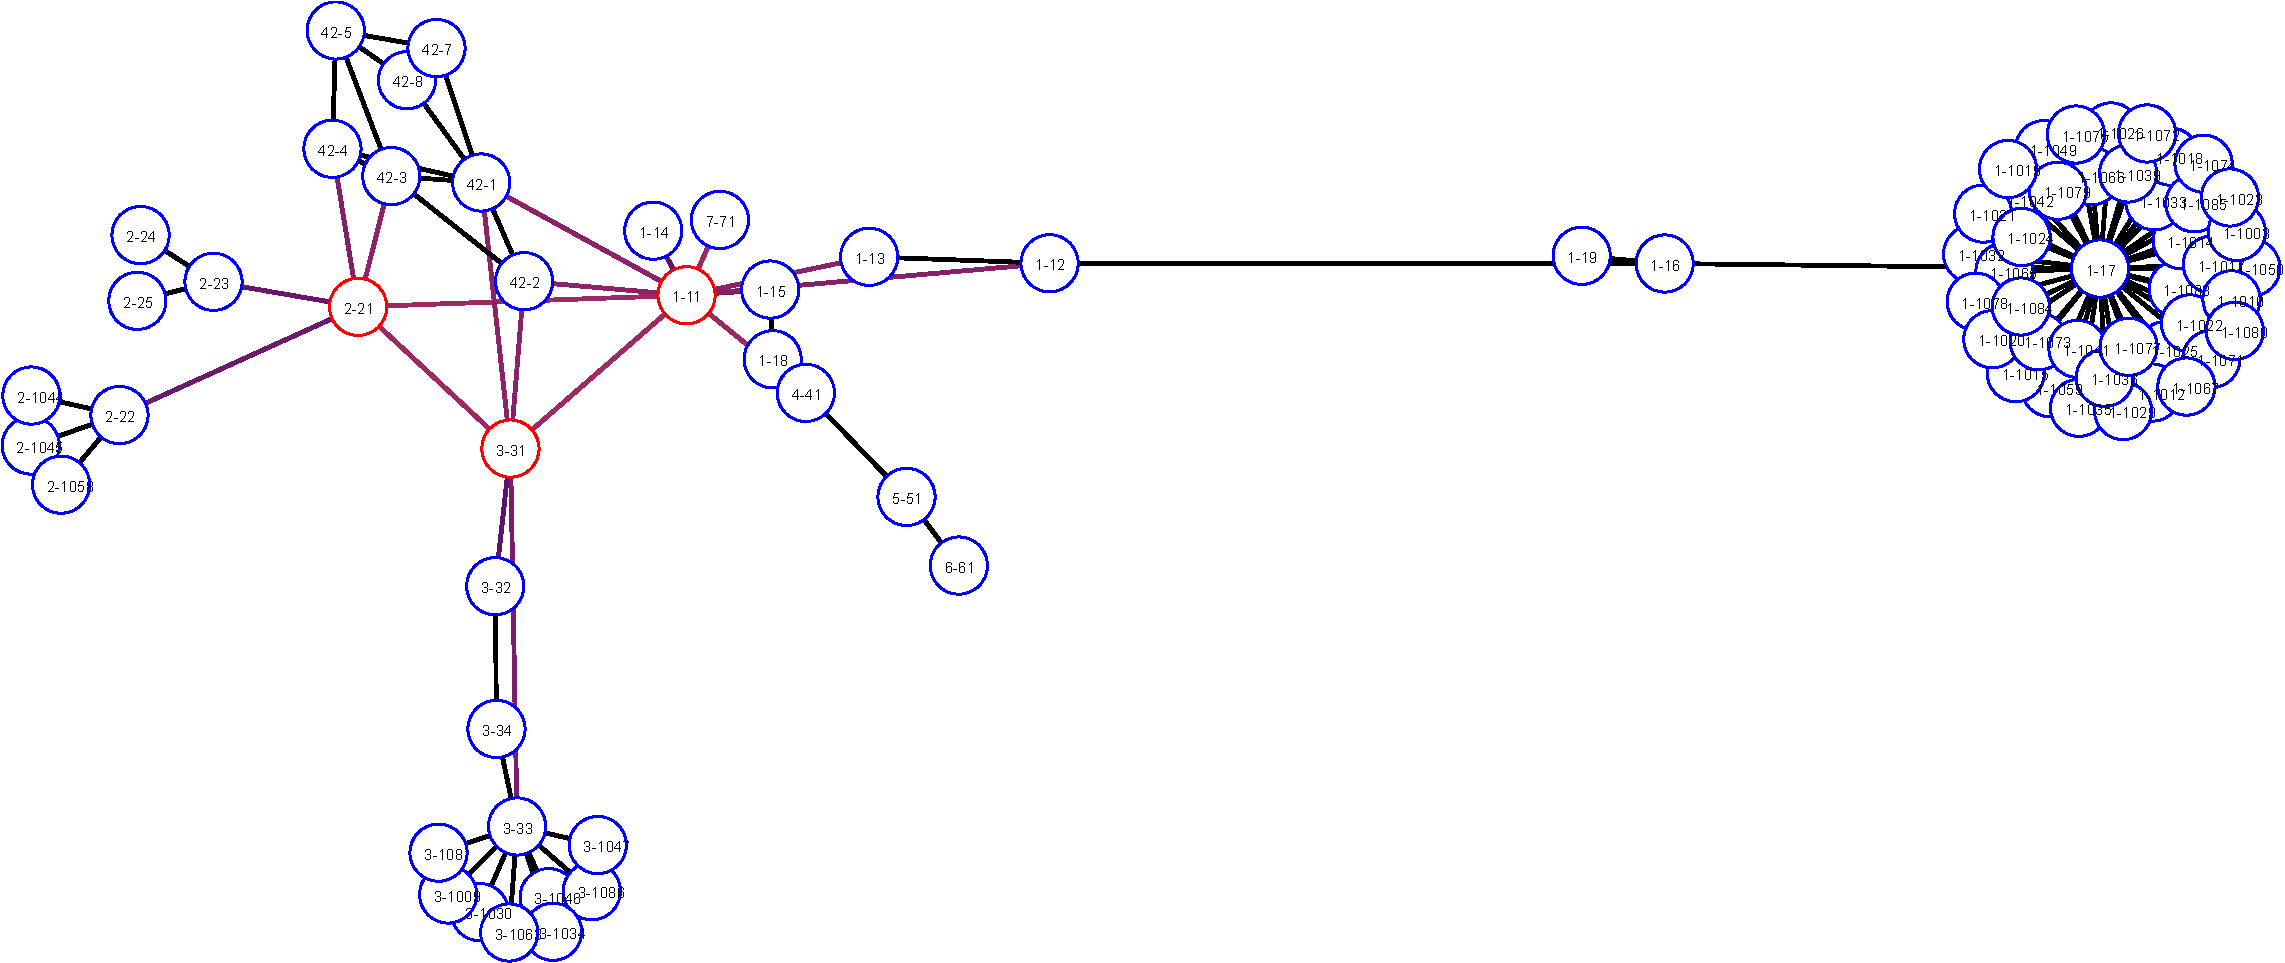
\includegraphics[width=.9\linewidth]{scionLabTopology.pdf}
	\caption{Part of SCIONLab topology}
	\label{fig:eva:scionLabTopo}
\end{figure}

\section{Experiment}

The experiment was ran on the SCIONLab network over 48 hours and ran multiple configurations of the SpeedCam program simultaneously. The script and the start parameters can be found in \autoref{app:config} and differ from the standard configuration in its each instance. The standard weights all criteria equally with 1, start an inspection every 10 seconds and uses 20\% of the network nodes. They were set intuitively while developing the software and serve as a baseline. This configuration used a history of six episodes for each node. The other configurations are:

\begin{easylist}
	# \textit{Const} uses only one node as a SpeedCam and does not scale with the network. This shall show the inefficiency of such strategy for dynamic, unexplored networks like SCIONLab.
	# \textit{Linear01} uses 10\%, \textit{Linear033} 33\% of the network nodes and will be used the evaluate the different scale methods. \textit{Linear02} uses the standard values with 20\% linear scaling. The naming convention is based on the factor, Linear01 conforms to $0.1 \cdot n$ and the same for the other configuration.
	# \textit{Log} uses a logarithmic scale with the base of 10 to calculate the amount of SpeedCams. As already discusses it is expected to result in a lower precision than the linear scaling methods.
	# \textit{Random} waits a random time between an inspection to start a new one. The random interval is between 10 seconds (default) to one hour. In contrast to this \textit{fixex} waits always 60 seconds before starting a new inspection.
	# \textit{Experience} uses the strategy by using past inspection to predict the next one. \textit{Experience12} uses twice as much episodes (total of 12) and \textit{Experience03} uses half as much with a total of only 3 episodes. The experience strategy starts with the random strategy until there are 5 data points.		
\end{easylist}

Each instance writes the result of an inspection to a .JSON file containing the complete network graph with past episodes and also the result of the inspection run. 

A Prometheus server is additionally running to provide a baseline of the measured traffic inside the network. This instance fetch data from all border router in an interval of 15 seconds. The difference to the inspector is, that the Prometheus server fetches always the metrics. The data will be used to calculate the precision of the monitored data with \autoref{equo:qualitySelection}, where $\text{traffic}(N)$ is equals to the Prometheus server data. 

Because of the missing or irregular set capacity information a congestion could not be detected, but can only be guessed. This results in unverifiable cases of \autoref{tab:classifyUser}. Instead the hit rate of finding maximums is used to calculate the quality of a configuration. The result list of monitored ASes is sorted by their recorded bandwidth for both the inspector and the Prometheus server. When the inspector and the Prometheus Server has the same maximum, the inspection is considered a hit. To soften the possible error of differentiating the bandwidth at different points of time, the maximum is spanned to until the third position. If the Prometheus maximum AS is at the 2nd or even the 3rd position of the inspectors, the inspection could also be a hit, but a weaker one. This is considered by using a difference of 0, 1 and 2 from the top position and for each difference the hit rate is calculated. Beside that, when the top AS is too far away, the inspection is considered an a miss.

The performance influence of the inspector is measured with the UNIX tool \textit{top} and creates a snapshot of the memory and CPU usage of the programs every 5 seconds. It was build with Go 1.9.5 linux/amd64 without any additional flags and all configurations ran as parallel processes without influencing each other. The IO influence was not captured because the inspector writes only a JSON mostly fewer than 100 KB after an inspection. It is assumed that this has no impact on the overall performance and can even be disabled in a real application.

\section{Result}
This part will list the results of the previously described configuration. \autoref{fig:eva:monitoredTraffic} displays the traffic in the time of the experiment, \autoref{fig:eva:monitoredTraffic:input} for the input of the interfaces and \autoref{fig:eva:monitoredTraffic:output} for the output of the interface. The series \textit{prometheus} is the data from the Prometheus server and serves as the comparison. The difference in the behavior of this for the input and the output resides, that the monitored network is only a part of the SCIONLab and routed traffic flows inside the monitored than outside because of the presence of general attachment points. 

The figure even gives a good impression of the results and the influence of the configuration. The best configuration, \textit{linear033}, monitored only about 50\% of the total traffic, while random based strategies as the \textit{experience} ones has the worst coverage. This will be discussed in detail in \autoref{sec:eva:precision}.

\begin{figure}[h]
	\centering
	\begin{subfigure}{.8\linewidth}
		\centering
		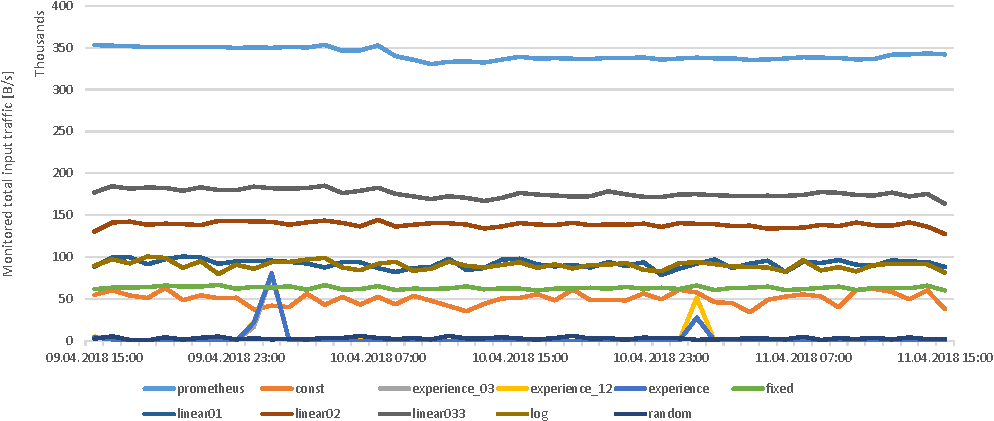
\includegraphics[width=0.98\textwidth]{monitoredTraffic_input.pdf}
		\caption{Input}
		\label{fig:eva:monitoredTraffic:input}
	\end{subfigure}
	\hfill
	\begin{subfigure}{0.8\linewidth}
		\centering
		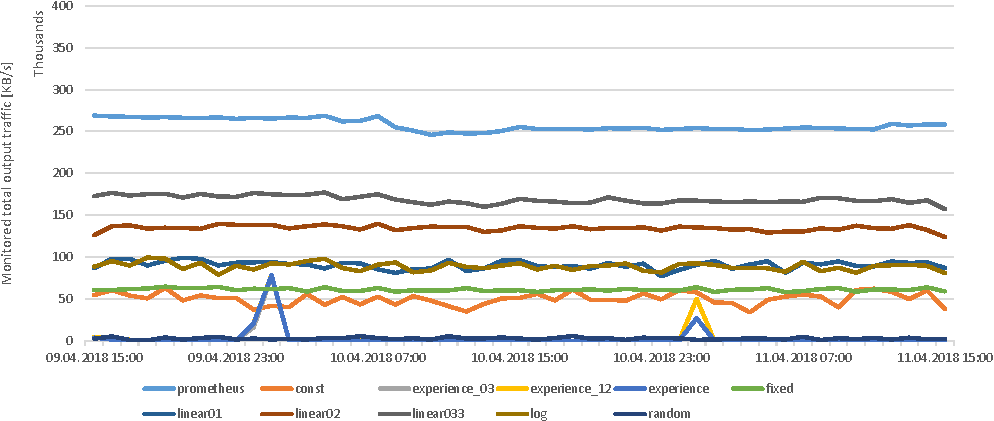
\includegraphics[width=0.98\textwidth]{monitoredTraffic_output.pdf}
		\caption{Output}
		\label{fig:eva:monitoredTraffic:output}
	\end{subfigure}
	\caption{Monitored bandwidth in bytes per second over the experiment time. Down sampled from 15 seconds to 1 hour.}
	\label{fig:eva:monitoredTraffic}
\end{figure}

One problem with the evaluation was to have only a partition of ASes with an accessible Prometheus client interface. The ratio is shown in \autoref{fig:eva:nodesRatio}. It displays the average amount of ASes the configuration has discovered, the candidates which has such an open client interface and the used SpeedCams per episode. \textit{random} has the lowest with 54 ASes, while \textit{fixed} has nearly twice of 102 ASes discovered. The reason for it, that \textit{random} has very few inspections and has a small chance to react to changes of the network. Additionally, new ASes were not only discovered when the path requests contained them, but also when a SpeedCam return a border router result with an unknown AS. This happened a lot for the attachment point of the virtual machines, AS 1-17. While this did not have an influence on the candidates it will have one with an improved possibility to monitor traffic. One example would be a possibility without knowing the border routers URL. Details will be listed in \autoref{chap:concl}.

\begin{figure}[h]
	\centering
	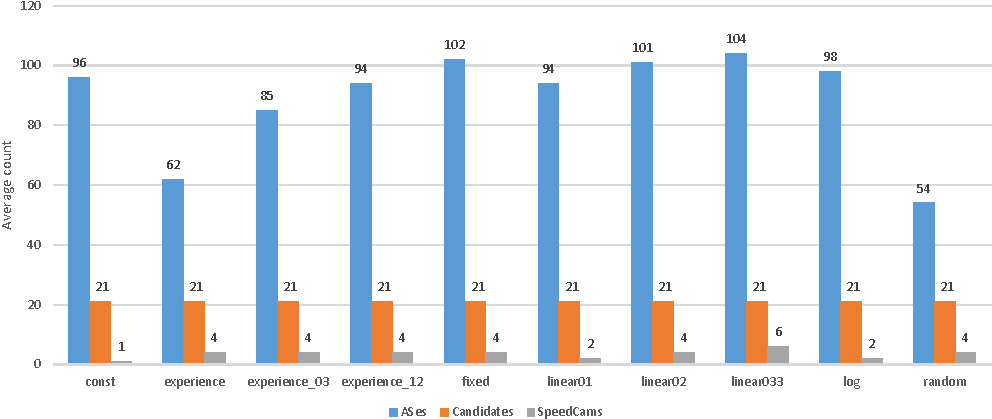
\includegraphics[width=.7\linewidth]{ASCandidateSpeedCamRatio.pdf}
	\caption{Average amount of discovered ASes, usable candidates and the used SpeedCams per configuration}
	\label{fig:eva:nodesRatio}
\end{figure}

\subsection{Precision} \label{sec:eva:precision}

The precision is the proportion of the real traffic by Prometheus to the monitored by the inspector. The higher the precision the better the inspection. It is split into the monitored input and output traffic and shown in separate graphs. The results are in percentage in \autoref{fig:eva:precisionPercent} where higher is better, but also in total difference in \autoref{fig:eva:precisionTotal} where lower is better.

Surprisingly the precision for the experience based strategies are zero in average, what means that the experience strategy do not cover any traffic in the network. The same result applies to \textit{random} and they are linked to each other. The experience strategy needs to gather a base of 5 data points and uses the random strategy for it and inherit the same result. Two possible solutions for this would be to use another training strategy or use a longer experiment duration instead of only two days. Alternatives are discussed in \autoref{chap:concl}. The left interval based strategy \textit{fixed} has a better result, but to far away from an acceptable distribution. It covers only 20\% in average and the very high variance are indicators, that a fixed inspection interval of one minutes can lead to many false-true classification because of low monitored traffic.

The other strategies are using an interval of 10 seconds between an inspection and vary in their amount of utilized SpeedCams. \textit{const} brings the worst results with a coverage of 10-20\%, but which is impressive for using only one node. It selected the core ASes \textit{1-14} 1564 times, \textit{3-31} 1019 times, \textit{4-41} 541 times and \textit{2-21} 381 times. Each of them is connected with the other ISDs and have high traffic, which is why there are selected so often. The \textit{const} strategy uses only 1 of 96 nodes to measure the traffic with a precision of 20\%.

The \textit{log} uses only one to two nodes more with an increase of 10\% points. A very similar picture is given by the \textit{linear01} scaling that happens because of the previously described problem with only 21 usable probes in the network. For that small number the scales differ only in on or two nodes. The other liner scales achieve a higher precision by using more nodes. Interesting is fixed and the linear configuration were able to monitor sometimes about 90 to 100\% of the network with a very small amount of nodes. The reason for that phenomena is that the selection consisted of very good probe points for the current flow. But this happened too few to be statistically relevant and should not be relied onto.

The same results can be viewed with the total difference in bytes per second in \autoref{fig:eva:precisionTotal}.

\begin{figure}[h]
	\centering
	\begin{subfigure}{.8\linewidth}
		\centering
		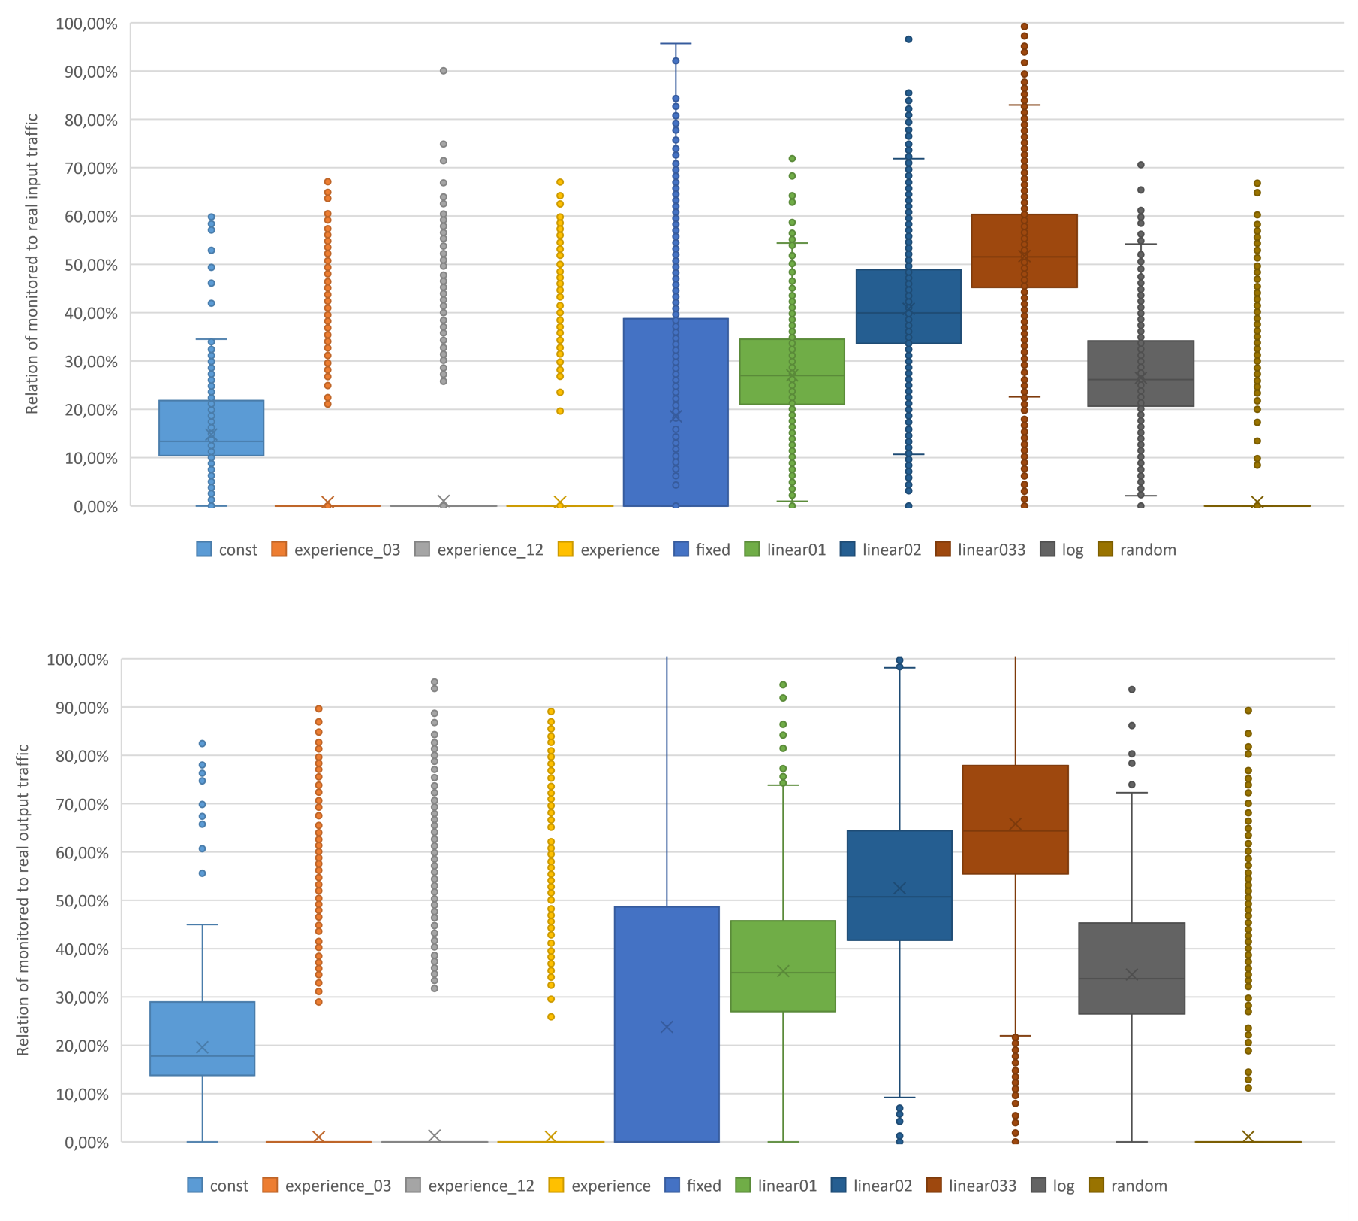
\includegraphics[trim={0mm 110mm 0mm 0mm},clip,width=0.98\textwidth]{percentageDifferenceTraffic_diagrams.pdf}
		\caption{Input}
		\label{fig:eva:precisionPercent:input}
	\end{subfigure}
	\hfil
	\begin{subfigure}{0.8\linewidth}
		\centering
		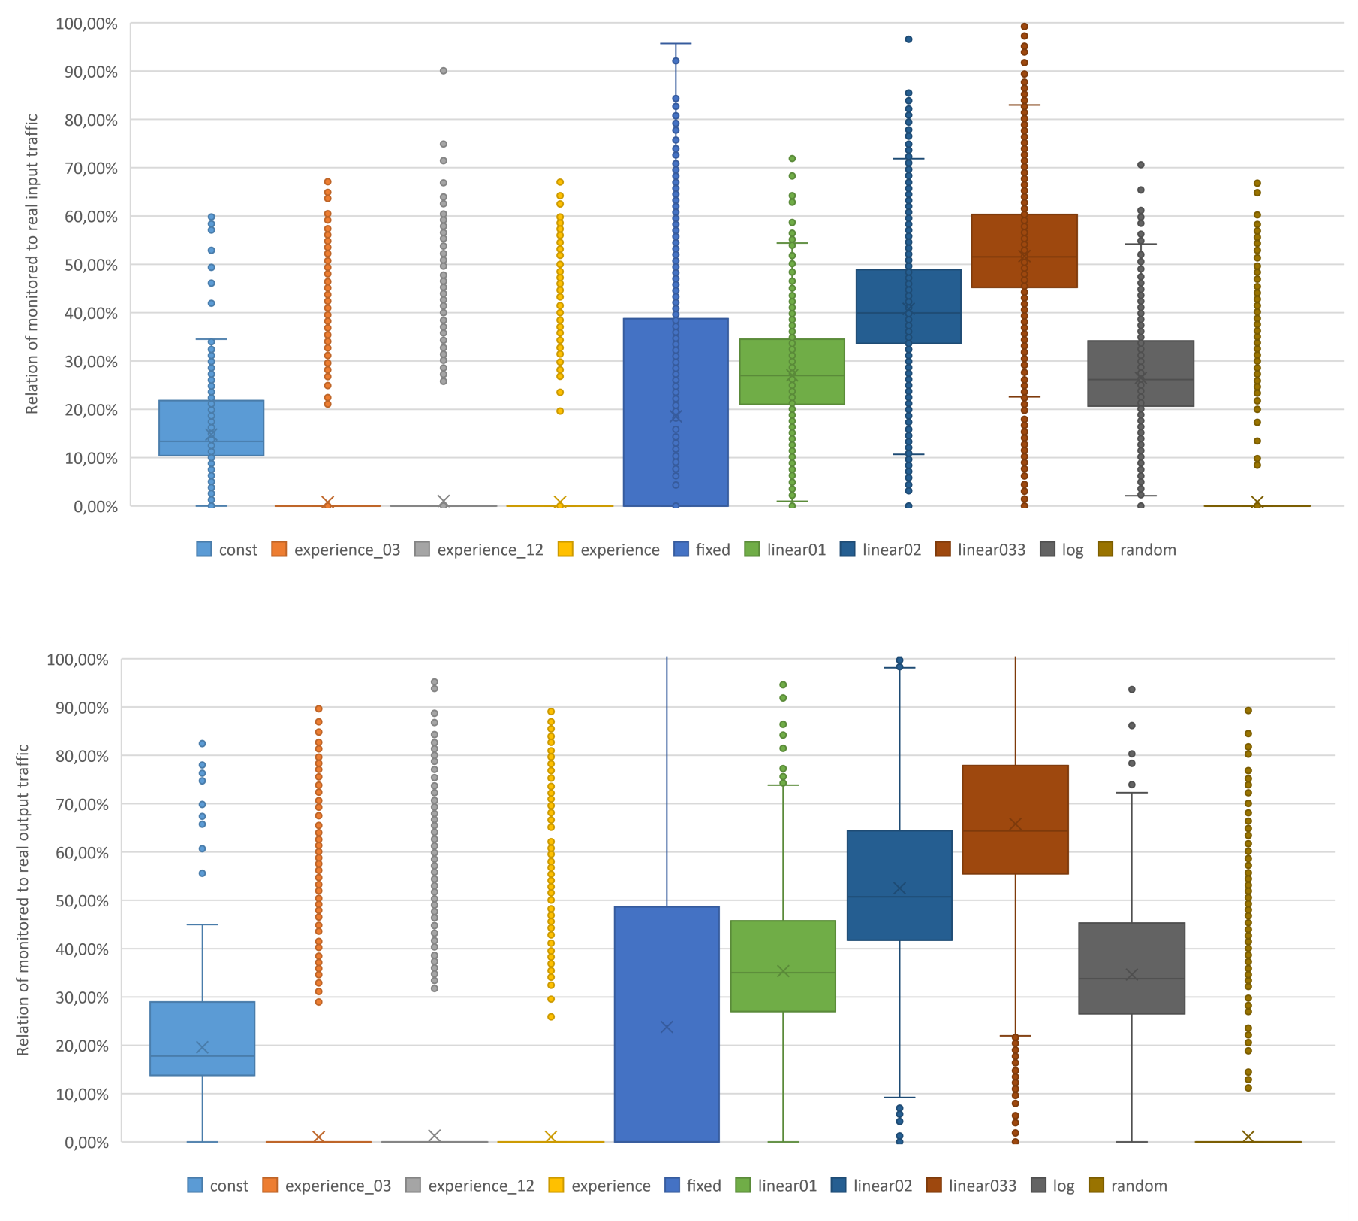
\includegraphics[trim={0mm 0mm 0mm 105mm},clip,width=0.98\textwidth]{percentageDifferenceTraffic_diagrams.pdf}
		\caption{Output}
		\label{fig:eva:precisionPercent:output}
	\end{subfigure}
	\caption{Distribution of percentage difference of real to monitored traffic}
	\label{fig:eva:precisionPercent}
\end{figure}

\begin{figure}[h]
	\centering
	\begin{subfigure}{.8\linewidth}
		\centering
		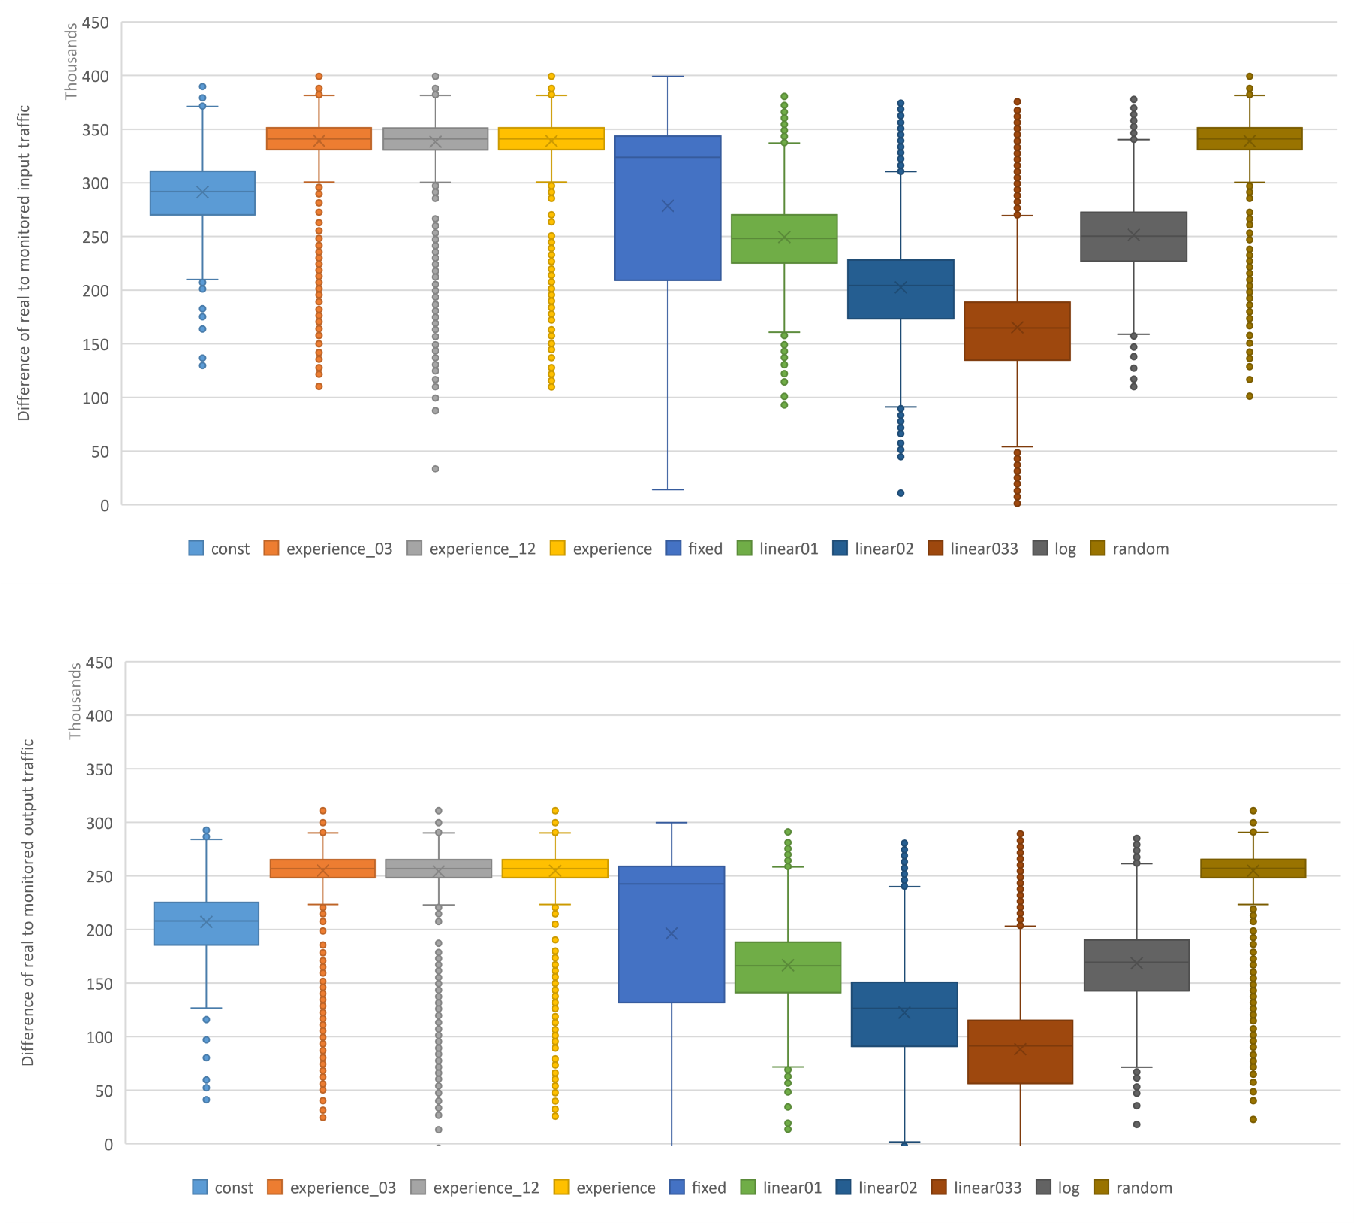
\includegraphics[trim={0mm 111mm 0mm 0mm},clip,width=0.98\textwidth]{totalDifferenceTraffic_diagrams.pdf}
		\caption{Input}
		\label{fig:eva:precisionTotal:input}
	\end{subfigure}
	\begin{subfigure}{0.8\linewidth}
		\centering
		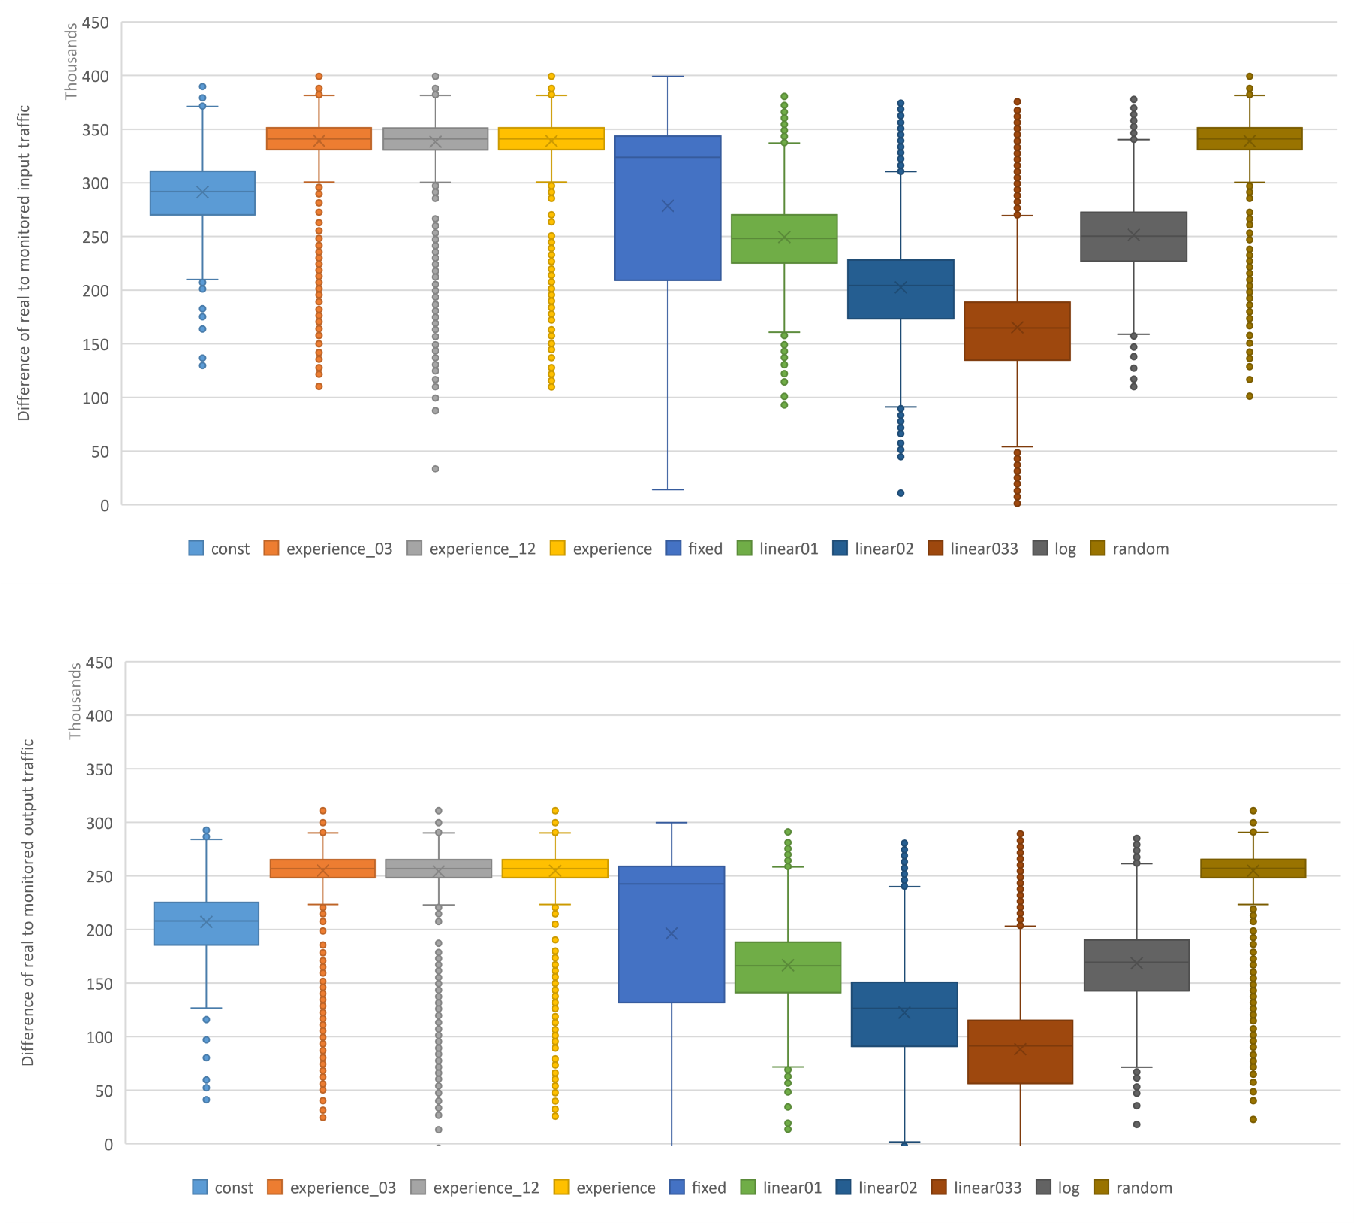
\includegraphics[trim={0mm 0mm 0mm 105mm},clip,width=0.98\textwidth]{totalDifferenceTraffic_diagrams.pdf}
		\caption{Output}
		\label{fig:eva:precisionTotal:output}
	\end{subfigure}
	\caption{Distribution of total difference of real to monitored traffic}
	\label{fig:eva:precisionTotal}
\end{figure}


\subsection{Hit and miss rate} \label{sec:eva:hitrate}
The hit and miss rate is an important criteria to rate a strategy. A high precision but a low hit rate indicates a bad decision of monitoring ASes. As previously discussed the hit rate will be examined with three different distances. The higher the distance the higher the error of a miss classified AS. The results are displayed in \autoref{fig:eva:hitrate}. Each diagram is split in the hit rate for the in- and the output because of the gab in the values as shown in \autoref{fig:eva:monitoredTraffic}.

The first observation of \autoref{fig:eva:hitrate} is that the hit rate is different for the input and the output estimation of the inspector. The exact reason for this phenomena is unclear and needs further investigations. An educated guess would be that because of the smaller gab between the real traffic and the monitored on the output interfaces (see \autoref{fig:eva:monitoredTraffic:output}) results in a smaller error in identifying the maximum bandwidth ASes.

The hit rate of an exact hit is for the input so low that every configuration identified the wrong AS as the one with the most bandwidth usage. The result for the output is much better, so that the fixed interval based configuration, the \textit{linear} ones, \textit{const} and \textit{fixed} itself, hat an exact hit at 25\% to 78\% of the time. The difference between \textit{fixed} and the other is that it uses a much longer interval between inspection (60s instead of 10s). This results in much more misses over the time because it doesn't run an inspection when Prometheus captures the traffic every 15 seconds. As seen in the different result of \textit{const} with only one SpeedCam and the other scaling strategies the amount of probes does have a positive impact on the hit rate. 

The hit rate increased when extending the acceptance range. Instead of an exact hit, a second or even third place is considered a hit. As seen for the linear configuration for the input, the increase is nearly 80\% points, \textit{const} increases by 50\% points and \textit{fixed} by 40\% points. An increase, but not so high, is seen for the output guess. An increase of the hit distance results in a correct guess for 50\% off the time for all but one not random based strategy. These are increasing, but only by a small amount.

Finally, the hit rate increases even further by extending the range by another 1. The linear configurations are now guessing the correct AS in 95\% of the time. This means, that the inspector with an interval of 10s and an amount of 2-6 probes in a network of about 100 ASes had identified the correct top three bandwidth user. Even using only one probe as seen in \textit{const} results in a high hit rate with that wide range.

All in all, it can be assumed that the hit rate depends primarily on a small inspection interval and secondarily on the amount of used probes.
\begin{figure}
	\centering
	\begin{subfigure}{0.8\linewidth}
		\centering
		\includegraphics[width=0.95\textwidth]{hitrateDist0.pdf}
		\caption{Distance 0 - Exact hit}
		\label{fig:eva:hitrate:0}
	\end{subfigure}
	\hfill
	\begin{subfigure}{0.8\linewidth}
		\centering
		\includegraphics[width=0.95\textwidth]{hitrateDist1.pdf}
		\caption{Distance 1 - 1st or 2nd}
		\label{fig:eva:hitrate:1}
	\end{subfigure}
	\hfill	
	\begin{subfigure}{0.8\linewidth}
		\centering
		\includegraphics[width=0.95\textwidth]{hitrateDist2.pdf}
		\caption{Distance 2 - 1st, 2nd or 3rd}
		\label{fig:eva:hitrate:2}
	\end{subfigure}
	\caption{Hit and miss rate of the inspection result over time. A hit occurs when the inspector top bandwidth consuming AS is the same as the Prometheus one.}
	\label{fig:eva:hitrate}
\end{figure}


\subsection{Performance} \label{sec:eva:performance}

The performance impact of SpeedCam on the system is minimal as seen in \autoref{fig:eva:performance}. Without the outliers, no configuration uses more than 1\% of the CPUs computation time and uses in average fewer than 0.5\%. The main impact of the CPU is the amount of utilized SpeedCams as seen in the linear configuration. The more SpeedCams existing, the more candidate scores needs to be calculated and the more monitoring results needs to get parsed. The random and the experience based configuration uses the fewest CPU in average, because most of the time they are sleeping and do not utilize the CPU.

The memory impact has a similar image as seen in \autoref{fig:eva:performance:mem}. No configuration needed more than 1.5\% of the memory. The amount of episodes per node has little to zero influence of the memory as seen for the experience configuration. A higher influence is the amount of used SpeedCams as seen for the \textit{const} configuration with always 1 SpeedCam, which uses nearly constant 1.1\% of the memory.

All in all does have no configuration a significant impact on the systems performance for the SCIONLab network. The goal was to use 5\% or fewer resources, which was achieved.
\begin{figure}
	\centering
	\begin{subfigure}{0.8\linewidth}
		\centering
		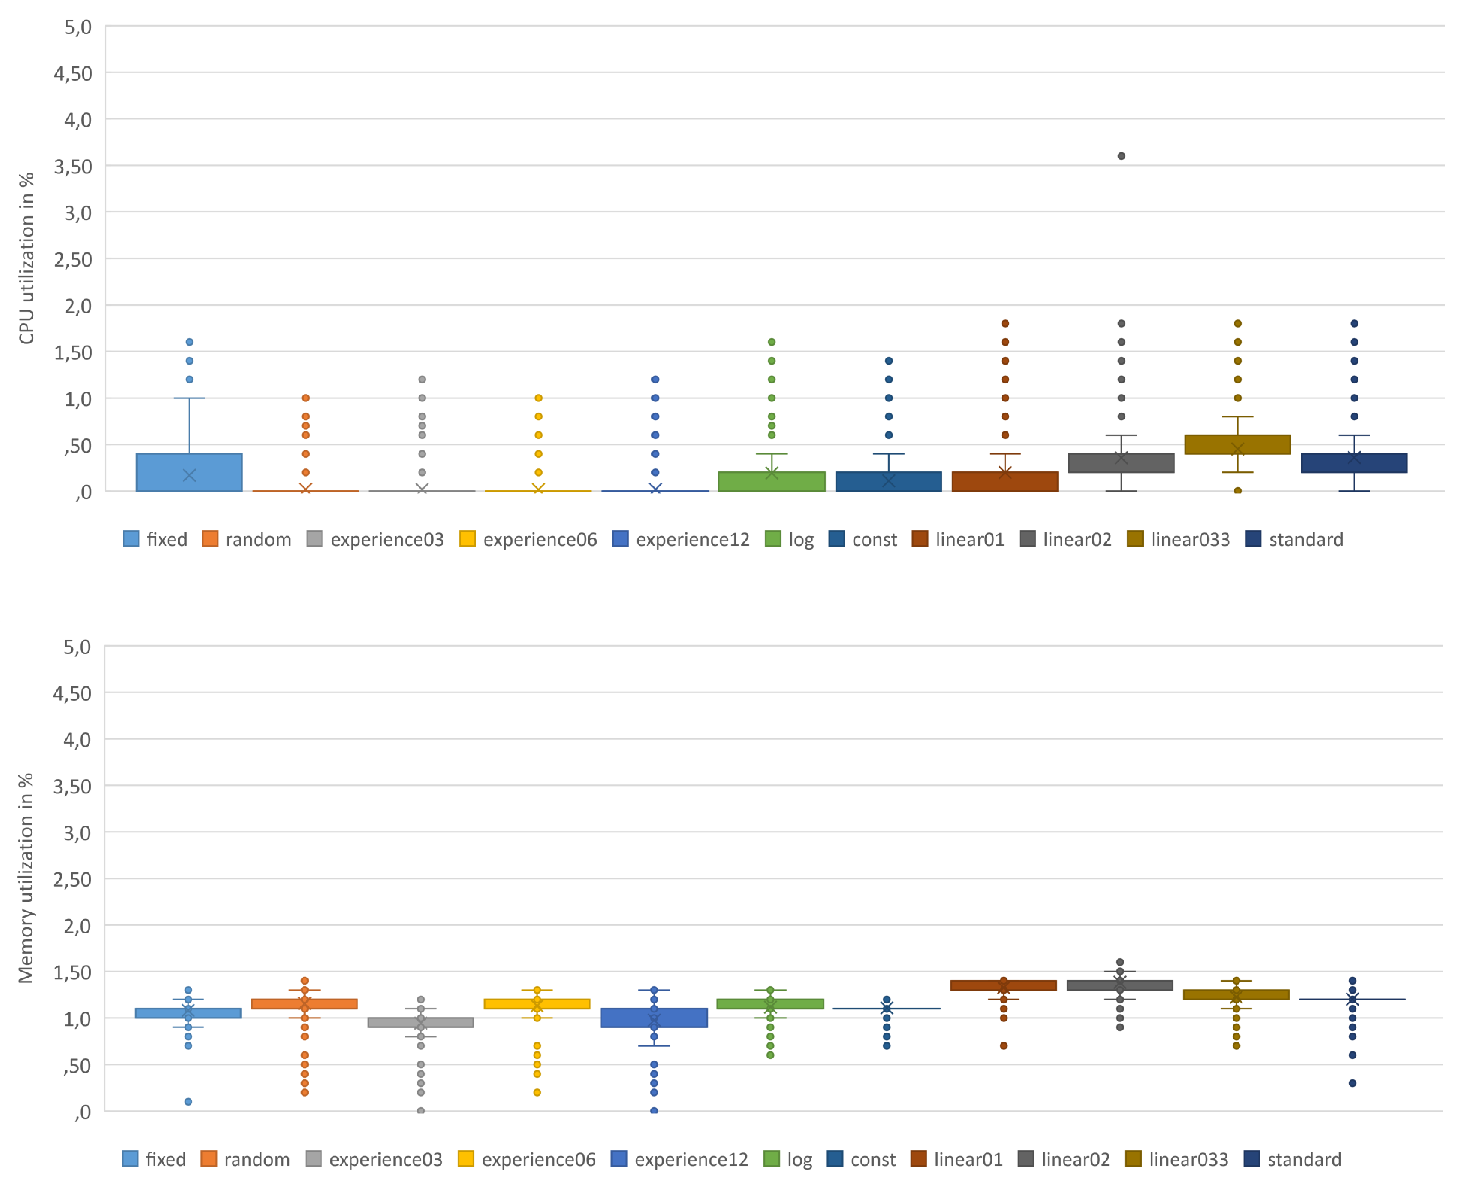
\includegraphics[trim={0mm 100mm 0mm 0mm},clip,width=0.98\textwidth]{performance_diagrams.pdf}
		\caption{CPU usage in \%}
		\label{fig:eva:performance:cpu}
	\end{subfigure}
	\hfill
	\begin{subfigure}{0.8\linewidth}
		\centering
		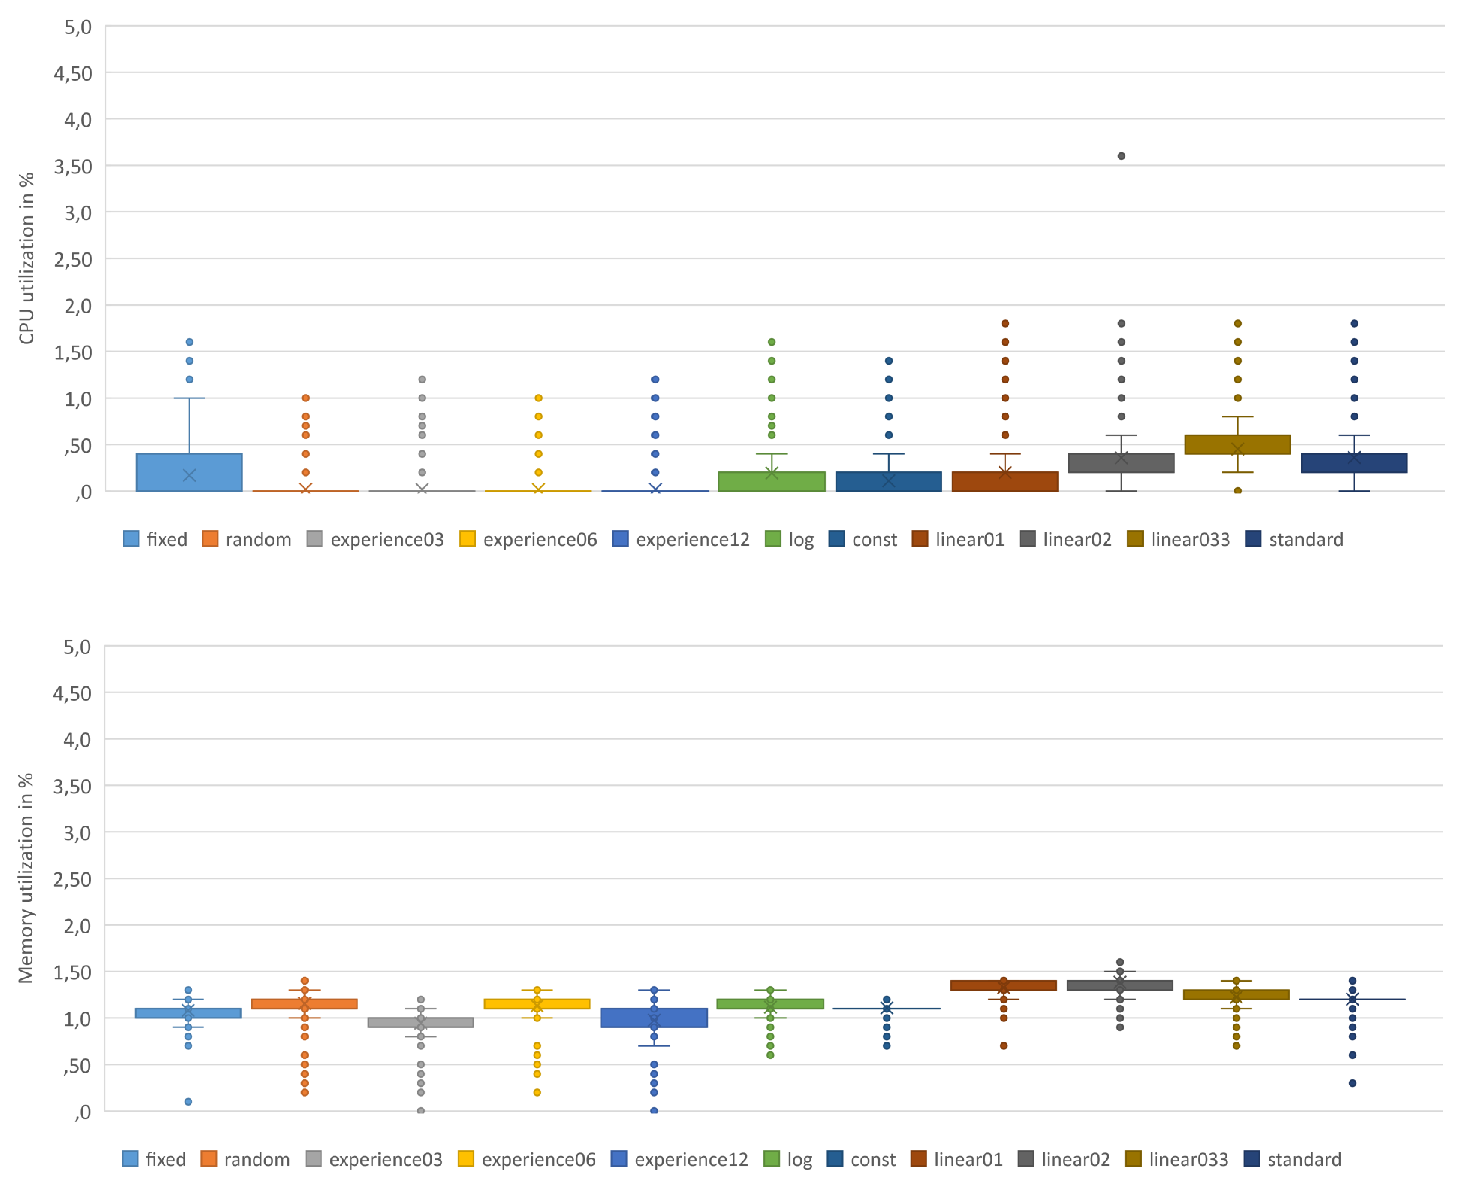
\includegraphics[trim={0mm 0mm 0mm 100mm},clip,width=0.98\textwidth]{performance_diagrams.pdf}
		\caption{Memory usage in \%}
		\label{fig:eva:performance:mem}
	\end{subfigure}
	\caption{Performance impact per configuration over 48h with a snapshot every 5s}
	\label{fig:eva:performance}
\end{figure}

\subfilebib % Makes bibliography available when compiling as subfile
\end{document}